\chapter{Background} \label{Related Work}
\ifpdf
    \graphicspath{{chapter_2/figures/PNG/}{chapter_2/figures/PDF/}{chapter_2/figures/}}
\else
    \graphicspath{{chapter_2/figures/EPS/}{chapter_2/figures/}}
\fi
%Write two to five lines about this chapter. 

\section{Introduction}
In this section, we present a brief literature review on predictive tools for anticancer peptide prediction and attribute of other biological attributes and processes.
\section{Existing Work and Web on Biological Entities}
We have studied some already developed project tools, there are some works for predicting biological entities like The first computational method to formulate anticancer peptide prediction as a machine learning problem was by Tyagi et al. in \cite{tyagi2013silico}. In their work, Tyagi et al. used amino-acid composition and binary profiles as input vectors and Support Vector Machines as the operating engine for classification. However, Vijaykumar et al. \cite{vijayakumar2015acpp} proved that on the dataset used by Tyagi et al. there were no significant difference among anticancer peptides and non-anticancer peptides in terms of amino-acid composition. Hence they proposed new effective features based on protein relatedness of amino acid distribution. They too used Support Vector Machines as classification algorithm.

In another work, Hajisharifi et al. \cite{hajisharifi2014predicting} used Support Vector Machines with Chou's pseudo-amino acid composition as input features. Later, Chen et al. proposed iACP \cite{chen2016iacp} that used g-gapped dipeptide composition as feature vector and Support Vector Machines as classification algorithm. In a very recent work, Wei et al. \cite{wei2018acpred} also used Support Vector Machines and employed binary profiles, amino-acid composition, g-gapped dipeptide composition, composition-transition-distribution based features and used feature selection to provide a web server that produces the so far best results. They also introduced a new updated benchmark dataset for training purpose. One thing to note that, most of these methods use single classifier which is Support Vector Machine in this case and uses wide range of feature vectors. All of them provides web servers for use. Ensemble based classifiers based on feature subspacing are previously used in solving drug-target interaction prediction \cite{rayhan2018cfsboost} and promoter identification problems \cite{rahman2018ipromoter}. Other ensemble based classifiers like Random Forest and Adaboost are also used for solving various related problems \cite{jani2018irecspot,rahman2018dpp}.
 
SPRINT-Mal and AntiCancer peptide prediction(ACPred-FL) are example of prediction tool. Sprint-Mal predicts lysine malonylation of sites of proteins using sequence and predicted structural features. It can predict lysine malonylation of sites of proteins from the protein sequence of Human and mouse \citep{Anderson04}. Anti cancer peptides works with two different dataset. One is to train the model and another one is to rest results. The training dataset is balanced. At predicts or classifies anti cancer peptides from protein sequence \citep{Anderson05}.\\
http://sparks-lab.org/server/SPRINT-Mal/  \\
server.malab.cn/ACPred-FL/ 

\begin{figure}[H]
  \centering
  \begin{minipage}[b]{0.4\textwidth}
    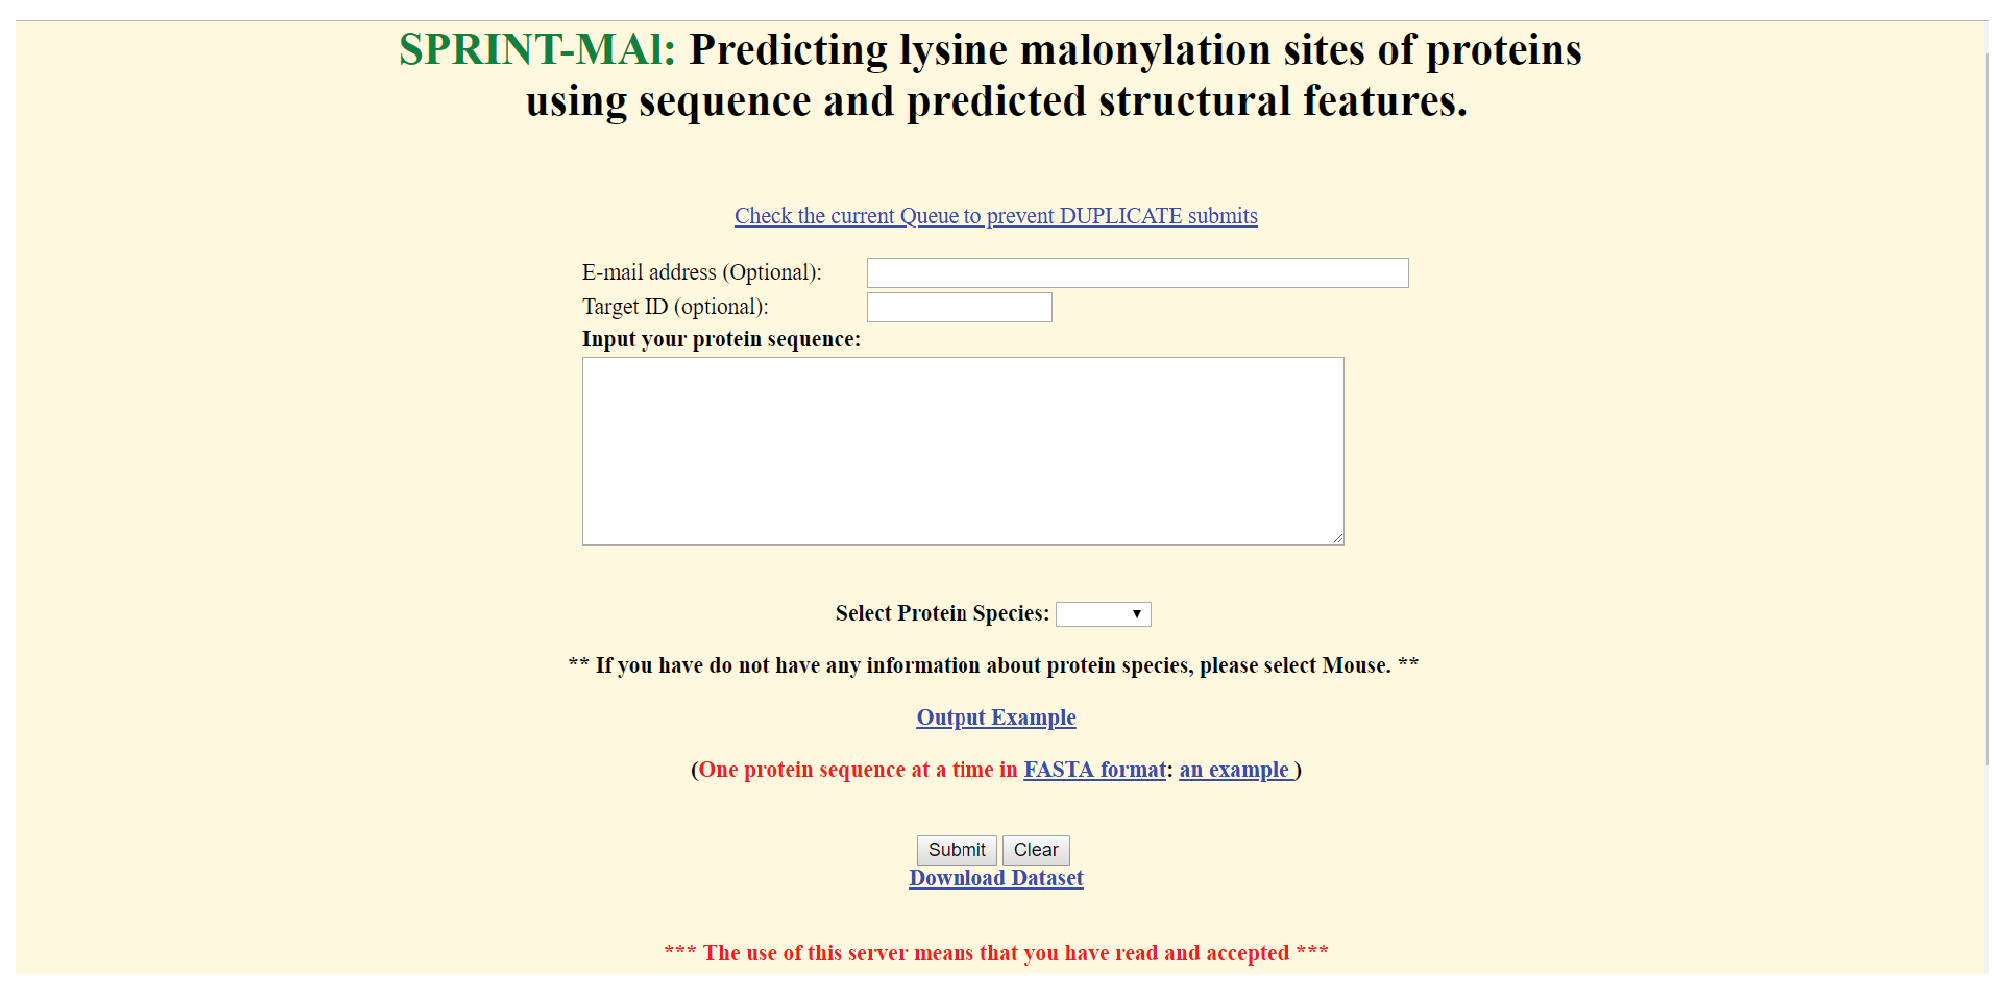
\includegraphics[width=\textwidth]{spintmal.eps}
    \caption{SPRINT-Mal}\centering \cite{Anderson04}
  \end{minipage}
  \hfill
  \begin{minipage}[b]{0.4\textwidth}
    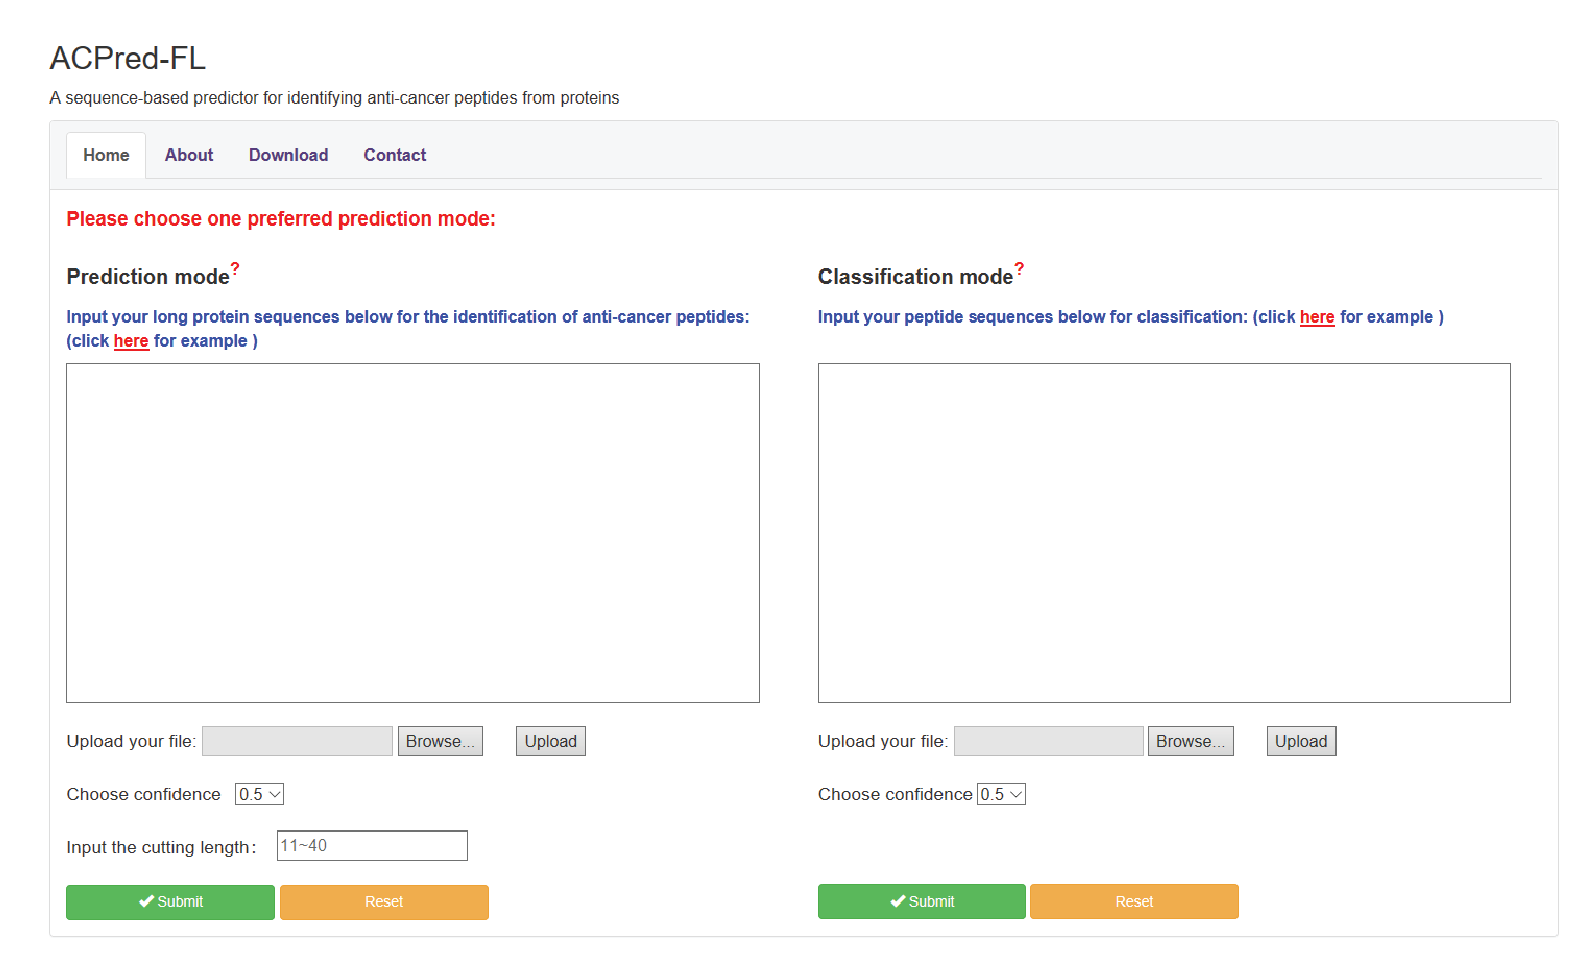
\includegraphics[width=\textwidth]{Anticancer.eps}
    \caption{ACPred-FL} \centering \cite{Anderson05}
  \end{minipage}
\end{figure}

\section{Comparison of Recent Workable Tools}
We have found some difference, when we studied the tools. Some comparison between the tools are given below :
\begin{table}[htbp]
\caption[Comparison of Recent Workable Tools]{Sprint-Mal \& ACPred-FL }
\centering
\footnotesize
\resizebox{\textwidth}{!}{\begin{tabular}{|c| >{\centering\arraybackslash}p{4.5cm} | >{\centering\arraybackslash}p{4.5cm} |} \hline
\bf No. & \bf Sprint-Mal & \bf ACPred-FL \\\hline
1. & There is option to input as mail for tracking user & There is option to take any input for tracking user  \\\hline
2. & There are some rule and regulation & There is no rule and regulation \\\hline
3. & It works on two data set so there is a choice option of prediction & It works only one data set so there is no option \\\hline
4. & There is only one option of prediction & There is two option for Identification and prediction  \\\hline
5. & There is no option to set up confidence level & There is option of choose confidence level  \\\hline

\end{tabular}}
%\label{training_testing_examples_KDD99}
\end{table}

\section{Software Requirement Specification (SRS)}
This document lays out a project plan for the development of "A tool for Prediction of Anticancer Peptide Using Sub spacing Ensemble Classifier". The plan will include, but is not restricted to a summary of the system functionality, the scope of the project from the perspective of the "Anticancer Prediction Problem" team (me, my team members and my supervisor), scheduling and delivery estimates, project risks and how those risks will be mitigated, the process by which we will develop the project will be recorded throughout the project.
\subsection{Overview}
Anticancer Peptide Prediction using laboratory method is time consuming and expensive. With laboratory method prediction is fully dependent on laboratorians and financial capabilities of individuals. We aim to develop an application that would enable them to save their valuable time and money with nearly perfect prediction system.
\subsection{Purpose}
The purpose of SRS document is to present a detailed description of constraint of anticancer prediction. It will explain the purpose and features of our system used here and how the system will work, what type of algorithms will be used here and how this system will be operated. This document is intended for both stakeholders and developers of the system.
\subsection{Scope}
In our system anticancer peptides prediction can be hazard free and cheap. Biologists spends their valuable time and laboratory resources for the prediction of anticancer peptides. Those methods are highly expensive. Our system will help them to predict anticancer peptides absolutely free. Thus will help them to invent cure for cancer patients.
\subsection{Goals}
After the completion of this project we aspire to fulfill some specific goals. Some of the goals are listed below. 
\begin{itemize}
\item Predict anticancer peptide using our developed tool
\item Help biologists/clinical researcher in the field of finding cancer cure
\item Reducing the cost of anticancer peptide prediction
\item Help saving time of researchers/biologists
\end{itemize}
\subsection{Overall Description}
Here we have described the overall process elaborately to provide as much as information about our project we can in an organized way.
\subsubsection{Users}
There will be mainly two kind of users of our web tool who are Clinical Researcher and Biologists.
\subsubsection{Functionality}
It is important to understand how our web tool will function. Down below we have listed the functionality of our web tool.
\begin{itemize}
\item User would be able to predict anticancer peptides 
\item User will provide protein sequence and our tool will predict attribute according to that
\item After prediction, predicted result will be shown to the user as a response message.
\end{itemize}
\subsubsection{Platform}
Our project will be launched as a Web-based application which will be accessed by a web browser which has an internet connection.
\subsubsection{Development and Responsibility}
We would be developing the software and we are responsible for the creation of related interfaces, server connections and support.
\subsubsection{Functional Requirements}
The functional requirement is describing the behavior of the system as it relates to the system's functionality. A finely designed system's usability is always satisfactory. This anticancer peptides prediction systems portal and each of its pages are very much easy to use. User will find it comfortable and some good set of directives are given to guide the user doing different set of activities. The category of user interfaces depends on the privileges given to the users. All the basic user functions that the user can perform are shown at the homepage and they are just one click away to access those functions. Making it user friendly is one of our prime goals and there will be a feedback screen for the user if there are any issues to address.

\paragraph{Step-By-Step Description:}
Clinical researchers or biologists uses the web tool to predict anticancer peptides. 
\begin{figure}[H]
\centering
 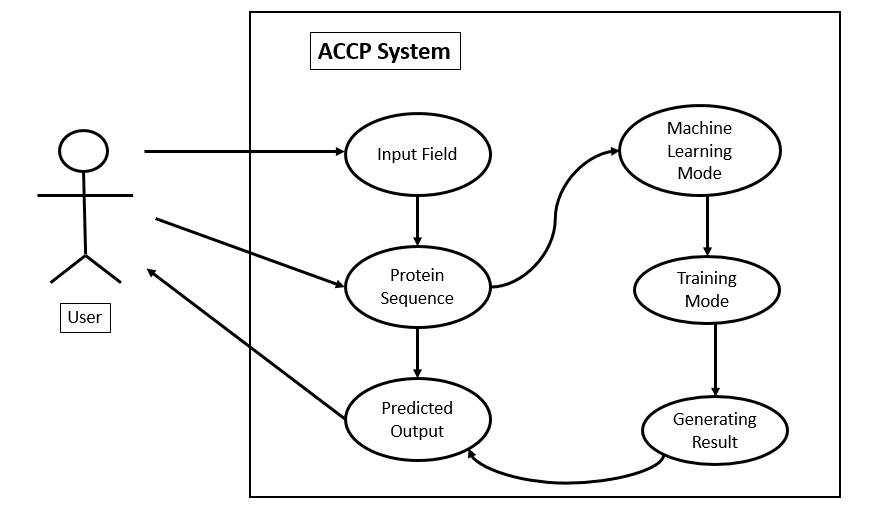
\includegraphics[width=0.7\textwidth]{useCase.PNG}
 \caption{Use Case Diagram of SRS}
 \label{fig:useCase}
\end{figure}
Use case diagram \ref{fig:useCase} also given which help us to visualize the whole process.
\begin{itemize}
\item Researchers/Biologists/User inserts protein sequence in the text field
\item That sequence is sent to the machine learning algorithm
\item Machine learning algorithm predicts anticancer peptide based on previously saved trained model
\item Prediction result is show to the user/researchers/biologists after predictions.
\end{itemize}

\subsubsection{Requirements Specification}
Let us discuss the non-functional requirements of our routine management system.
\paragraph{System Properties :}
The system properties are listed below which describes which tools were used to make this project and what are the requirements to run this tool.

\begin{description}
\item[(a)] A web based anticancer peptides prediction system runs on the internet
\item[(b)] Runs on Linux server
\item[(c)] HTML/CSS, Bootstrap, JavaScript based UI design
\item[(d)] Python flask based functioning system.
\end{description}
\paragraph{Storage Requirements :}
The storage requirements for the project are described down below.
\begin{description}
\item[(a)] Different contents uploaded to the system are preserved
\item[(b)] Minimum and maximum requirements of disk space are considered with care
\item[(c)] Unnecessary and obsolete contents are removed to free the disk space.
\end{description}
\paragraph{Accessibility :}
Here we have stated the means by which someone can access this web tool.
\begin{description}
\item[(a)] This system is accessible from mobile/desktop/laptop devices
\item[(b)] A stable internet connection is required.
\end{description}
\paragraph{Documentation :}
Proper documentations make it easier to use any system. We will provide visual directions and instructions to use this web tool.
\begin{description}
\item[(a)] User guidelines to use the system with screen-shots will be provided
\item[(b)] User privileges and access management guidelines will be added in the documentation.
\end{description}
\paragraph{Availability :}
The system will be available to its specific users as stated below.
\begin{description}
\item[(a)] Any user can access this system 24/7
\item[(b)] A minimum amount of downtime will be taken during maintenance period.
\end{description}
\subsubsection{Technical Process}
Following would be the languages we would like to use for the development of our application within the stipulated time period.
\paragraph{Front-end development :}
HTML, CSS, Bootstrap, JavaScript.
\paragraph{Back-end development :}
\begin{itemize}
\item Programming Language : Python
\item IDE : Anaconda, Notepad++, Spyder
\item Virtual Machine : Vagrant Box. 
\end{itemize}

\section{Summary}
In this chapter we know about existing works and SRS. Which inspired us and helped us to develop our project.